\documentclass[11pt]{article}
\usepackage[a4paper, portrait, margin=1in]{geometry}
\usepackage{mathtools}
\usepackage{listings}
\usepackage[dvipsnames]{xcolor}
\usepackage{color}
\usepackage{graphicx}
\usepackage[colorlinks=true,urlcolor=blue,linkcolor=gray]{hyperref}


\DeclarePairedDelimiter{\ceil}{\lceil}{\rceil}

\newcommand{\code}[1]{\lstinline[language=Java]{#1}}
\newcommand{\todo}[1]{\fcolorbox{black}{Apricot}{TODO: #1}}
\newcommand{\linkmain}[1]{\href{https://gitlab.inf.ethz.ch/pungast/asl-fall16-project/blob/master/src/main/java/asl/#1.java}{#1}}
\newcommand{\linktest}[1]{\href{https://gitlab.inf.ethz.ch/pungast/asl-fall16-project/blob/master/src/test/java/asl/#1.java}{#1}}

\newcommand{\resultsurl}[1]{\href{https://gitlab.inf.ethz.ch/pungast/asl-fall16-project/blob/master/results/#1}{gitlab.inf.ethz.ch/.../results/#1}}




\begin{document}

\title{Advanced Systems Lab (Fall'16) -- Second
Milestone}

\author{Name: \emph{Taivo Pungas}\\Legi number: \emph{15-928-336}}

\date{
\vspace{4cm}
\textbf{Grading} \\
\begin{tabular}{|c|c|}
\hline  \textbf{Section} & \textbf{Points} \\ 
\hline  1 &  \\ 
\hline  2 &  \\ 
\hline  3 &  \\ 
\hline \hline Total & \\
\hline 
\end{tabular} 
}

\maketitle

\newpage

\section*{Notes on writing the report \small{(remove this page for submission)}}

Before starting to work on this milestone please remember:
\begin{itemize}
\item The prerequisite to a successful completion to this milestone is to have a stable system and also the necessary logging functionalities in place. 
\item Depending on the workload and goal of the experiment, you might need to change the sampling rate from the default level. Make sure to indicate when doing so.
\item The choice of experiment length and repetitions is up to you to decide, please make sure that you do not include warm-up and cool-down phases in the measurements. There are many experiments to run in this milestone, try to make a tradeoff.  
\item We recommend that you have scripts in place to deploy and run experiments.
\item All experiments have to be executed on the Microsoft Azure cloud.
\item When plotting graphs include errors or measures of accuracy whenever possible. 
\item Keep the report compact and concise! The total length should not exceed 20 pages. Log listings are not counted in this length, but all text, figures and tables are. If you have many logs, compress them by experiment and reference the archive instead of the independent files.
\end{itemize}

In this milestone we expect to see the different experiments you ran to exercise the system, and with each experiment we expect a clear description of the system configuration used, the hypothesis on behavior and the explanation of the behavior observed (in terms of the different design decisions taken beforehand) -- \emph{missing either of these for an experiment might make you lose all points for that given experiment!} 

Keep in mind that for a good explanation of the results of an experiment you might have to use one or more methods of data analysis presented in the lecture and in the book. You might have to combine measurements taken in the middleware with the ones at the clients to be able to provide a full picture.

Please feel free to structure the three sections of this report as it makes most sense for your experiments and explanations, but please respect the goal of each section. Also, similarly to the first milestone, include tables and descriptions about your experimental setup before each set of experiments.

\medskip

\pagebreak

% --------------------------------------------------------------------------------
% --------------------------------------------------------------------------------
\section*{Modifications to the middleware}
% --------------------------------------------------------------------------------
% --------------------------------------------------------------------------------
In the last milestone submission, my middleware implemented all functionality as necessary. However, the resource usage was extremely wasteful: each read thread took up nearly 100\% of the resources allocated to them and never went to a sleeping state. This caused more than 10-fold drops in performance when going from $T=1$ to $T=4$ (for $S=5$), and would have made the maximum throughput experiment useless. The changes can be seen on \href{https://gitlab.inf.ethz.ch/pungast/asl-fall16-project/commit/928e9bba132d34ecf9c00936babdd7fa2645e50f}{GitLab}.

To verify that the system is still stable, I re-ran the trace experiment. The throughput and response time are shown in Figures~\ref{fig:trace:throughput} and \ref{fig:trace:responsetime}, and are confirmed to be stable (and throughput is roughly 30\% higher). The Interactive Response Time Law also still holds (to within 0.46\%). For explanations of the figures, see Milestone 1 report.

\begin{figure}[h]
\centering
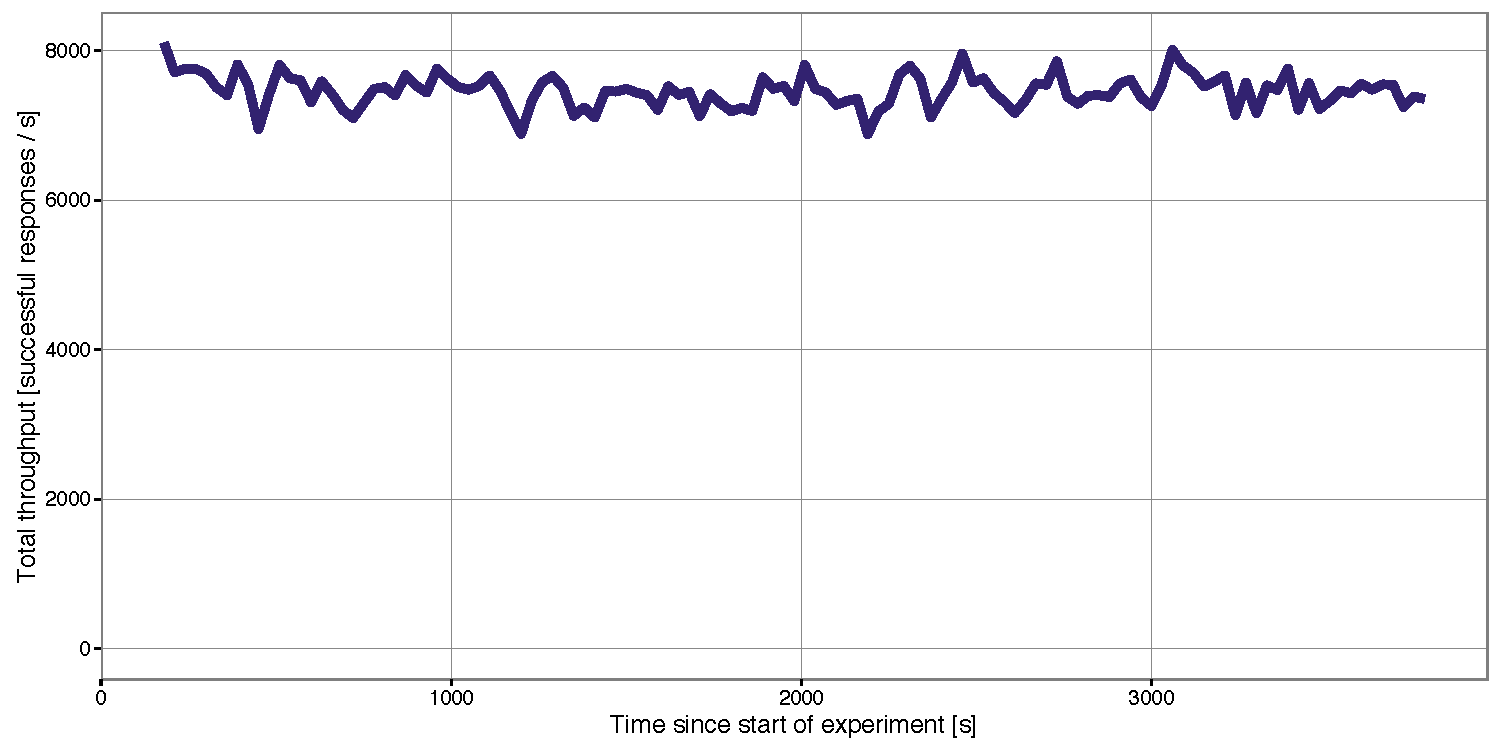
\includegraphics[width=\textwidth]{../results/trace_rep3/graphs/throughput.pdf}
\caption{Throughput trace of the middleware.}
\label{fig:trace:throughput}
\end{figure}

\begin{figure}[h]
\centering
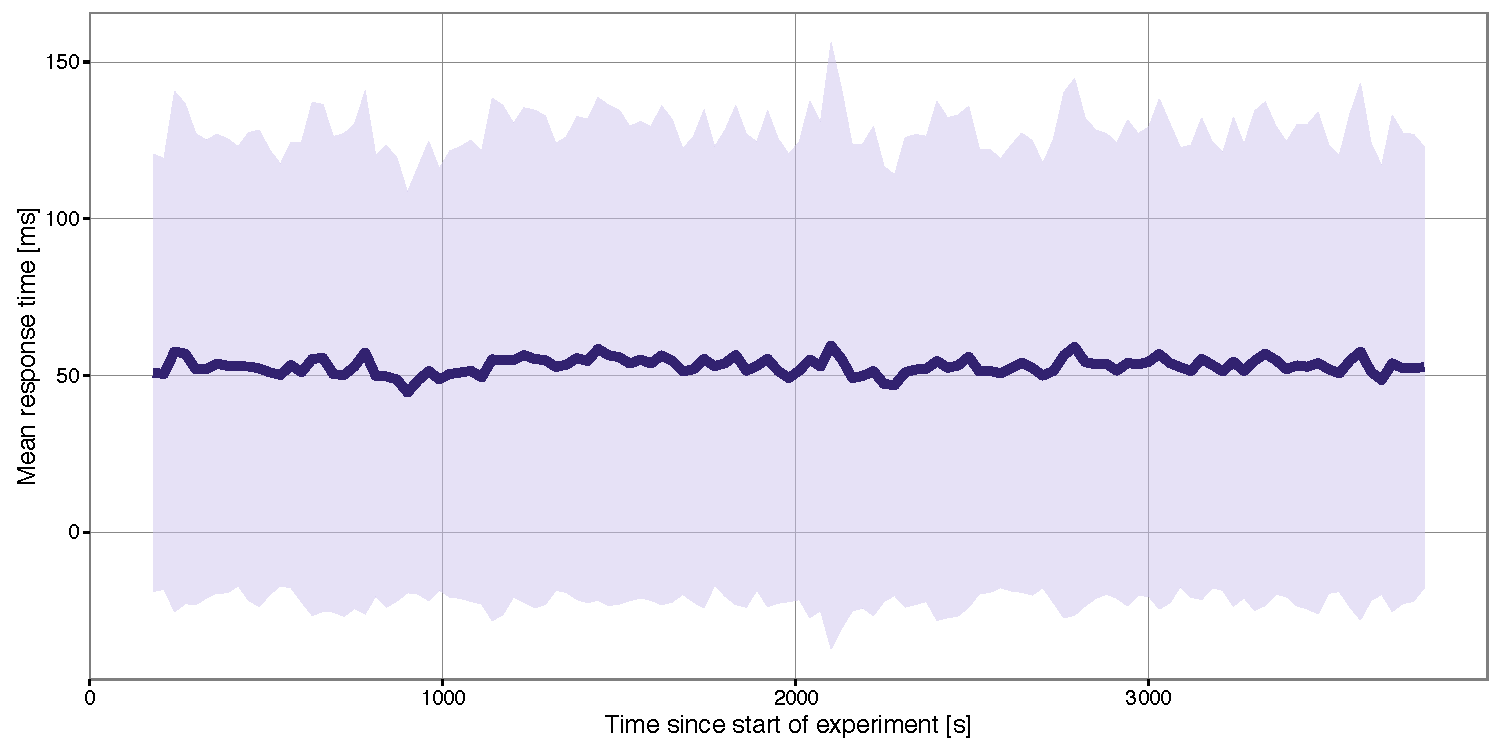
\includegraphics[width=\textwidth]{../results/trace_rep3/graphs/responsetime.pdf}
\caption{Response time trace of the middleware as measured by memaslap.}
\label{fig:trace:responsetime}
\end{figure}

% --------------------------------------------------------------------------------
% --------------------------------------------------------------------------------
\section{Maximum Throughput}
% --------------------------------------------------------------------------------
% --------------------------------------------------------------------------------

Find the highest throughput of your system for 5 servers with no replication and a read-only workload configuration. What is the minimum number of threads and clients (rounded to multiple of 10) that together achieve this throughput? Explain why the system reaches its maximum throughput at these points and show how the performance changes around these configurations.

Provide a detailed breakdown of the time spent in the middleware for each operation type.

\subsection{Experimental question}

The system under test (SUT), in this section and hereafter, is the middleware together with the memcached servers running on virtual machines in the Azure cloud.

In this section, I will run experiments to find out a) the maximum throughput of the SUT, b) the number of read threads ($T$) in the middleware that achieves this c) the number of virtual clients ($C$) that achieves this.

To this end, I will measure throughput (the number of requests the SUT successfully responds to, per unit of time) as a function of $T$ and $C$. I will find the maximum sustained throughput of the SUT, i.e. the throughput with which the response time does not increase rapidly with additional clients.

\subsection{Hypothesis}

I approximate that the maximum throughput will be 17200 requests per second using 50 read threads in the middleware at a load of 192 to 550 clients.

\paragraph{Number of threads} 
Given that requests spend most of their time ($\sim90\%$ in the trace experiment) waiting in the queue, increasing $T$ will increase throughput. If we reduce the queueing time by a factor of 10, it will no longer be the bottleneck (then waiting for memcached's response -- which takes $\sim9\%$ of response time in the trace experiment -- becomes the bottleneck). Assuming the time spent in the queue scales linearly with the number of read threads, we should increase $T$ 10-fold, i.e. $T=50$ maximises throughput.

\paragraph{Number of clients} Throughput will be maximised at roughly 110 virtual clients per memcached server, so 550 virtual clients in total. This is based on the fact that in the Milestone 1 baseline experiment, the throughput of a single memcached server without middleware saturated at around 110 virtual clients. It is likely to be an overestimate since the SUT here has an additional part (the middleware) and the baseline experiment did not measure sustained throughput, but 550 clients is a reasonable upper bound. As a lower bound we can use the number of clients in the trace experiment: $3 \cdot 64=192$.

\paragraph{Throughput} Since in the trace experiment, the throughput was roughly 10300 requests per second, we have a lower bound for the expected throughput. Naively assuming that the throughput of GET requests scales linearly with the number of servers $S$ would yield an expected throughput of $\frac{5}{3} \cdot 10300 = 17200$ requests per second. However, this does not take into account that we will also increase the number of threads (from $T=5$ in the trace experiment). Thus I expect the maximum sustained throughput to be definitely more than 10300 requests per second, and likely to be more than 17200 requests per second.

I predict that the graph of throughput as a function of the number of clients will be similar to Figure~\ref{fig:exp1:hyp:throughput}: rapidly increasing at first, then reaching the knee after which throughput growth is much slower, and then saturating. After saturation, the throughput may fall due to unexpected behaviour in the middleware.

\begin{figure}[h]
\centering
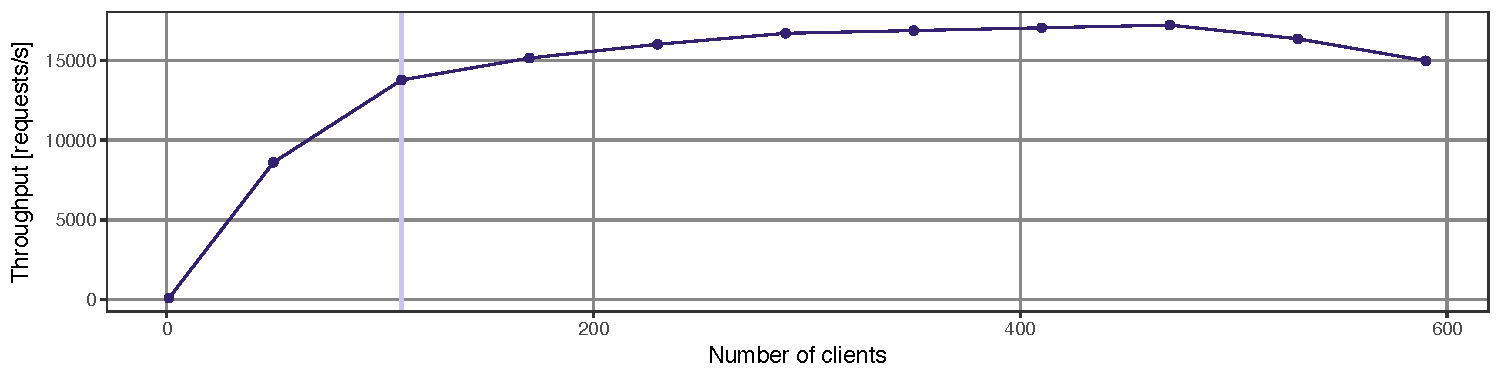
\includegraphics[width=\textwidth]{figures/hypothesis_throughput.pdf}
\caption{Expected graph of throughput as a function of number of clients (for the optimal value of $T$). The vertical line shows the optimal number of clients.}
\label{fig:exp1:hyp:throughput}
\end{figure}



\begin{itemize}
\item Draw graphs with expected results
\item Even try to predict variance and statistical properties
\item Make bullet points with explanations
\item Use „modeling“ to make hypothesis
\item Formulate a number of questions on what you expect to see, develop a hypothesis around the behavior that is expected, explain the hypothesis, and write it all down
\end{itemize}

\subsection{Experiments}
\begin{center}
\small{
\smallskip
\begin{tabular}{|c|c|}
\hline Number of servers & 5 \\ 
\hline Number of client machines & $\in \{1, 3\}$ \\ 
\hline Virtual clients & $\in \{1, 72, 144, 216, 288, 360, 432, 504, 576\}$ \\ 
\hline Workload & Key 16B, Value 128B, Writes 0\% \\
\hline Middleware: replication factor & 1 \\ 
\hline Middleware: read threads & $\in\{1, 16, 32, 64\}$ \\ 
\hline Runtime x repetitions & 6min x 1 \\ 
\hline Log files & \todo{} \\
\hline 
\end{tabular} }
\end{center}

Three client machines were used for all experiments, except for the 1-client experiment, where only one machine was used. The first 2 and last 2 minutes of each experiments were discarded as warm-up and cool-down time.

\subsection{Results}
Reporting experiment results. Comparison of hypothesis and experiment results.

% --------------------------------------------------------------------------------
% --------------------------------------------------------------------------------
\section{Effect of Replication}
% --------------------------------------------------------------------------------
% --------------------------------------------------------------------------------

Explore how the behavior of your system changes for a 5\%-write workload with S=3,5 and 7 server backends and the following three replication factors:
\begin{itemize} 
\item Write to $1$ (no replication) 
\item Write to $\ceil{\frac{S}{2}}$ (half) 
\item Write to all 
\end{itemize}

Answer at least the following questions: Are \texttt{get} and \texttt{set} requests impacted the same way by different setups? If yes/no, why? Which operations become more expensive inside the middleware as the configuration changes? How does the scalability of your system compare to that of an ideal implementation? Provide the graphs and tables necessary to support your claims.


\subsection{Experimental question}
\begin{itemize}
\item Define the „system(s) under test“
\item Define what to measure and understand why
\end{itemize}

\subsection{Hypothesis}
\begin{itemize}
\item Draw graphs with expected results
\item Even try to predict variance and statistical properties
\item Make bullet points with explanations
\item Use „modeling“ to make hypothesis
\item Formulate a number of questions on what you expect to see, develop a hypothesis around the behavior that is expected, explain the hypothesis, and write it all down
\end{itemize}

\subsection{Experiments}
\begin{center}
\small{
\smallskip
\begin{tabular}{|c|c|}
\hline Number of servers & $\in \{3, 5, 7\}$ \\ 
\hline Number of client machines & 3 \\ 
\hline Virtual clients / machine & \todo{} \\ 
\hline Workload & Key 16B, Value 128B, Writes 5\% \todo{} \\
\hline Middleware: replication factor & $\in \{1, ceil(S/2), S\}$ \\ 
\hline Middleware: read threads & \todo{} \\ 
\hline Runtime x repetitions & 60s x 5 \todo{} \\ 
\hline Log files & \todo{} \\
\hline 
\end{tabular} }
\end{center}

\subsection{Results}
Reporting experiment results. Comparison of hypothesis and experiment results.
 
% --------------------------------------------------------------------------------
% --------------------------------------------------------------------------------
\section{Effect of Writes}
% --------------------------------------------------------------------------------
% --------------------------------------------------------------------------------

In this section, you should study the changes in throughput and response time of your system as the percentage of write operations increases. Use a combination of 3 to 7 servers and vary the number of writes between 1\% and 10\% (e.g. 1\%, 5\% and 10\%). The experiments need to be carried out for the replication factors R=1 and R=all.  

For what number of servers do you see the biggest impact (relative to base case) on performance? Investigate the main reason for the reduced performance and provide a detailed explanation of the behavior of the system. Provide the graphs and tables necessary to support your claims.


\subsection{Experimental question}
\begin{itemize}
\item Define the „system(s) under test“
\item Define what to measure and understand why
\end{itemize}

\subsection{Hypothesis}
\begin{itemize}
\item Draw graphs with expected results
\item Even try to predict variance and statistical properties
\item Make bullet points with explanations
\item Use „modeling“ to make hypothesis
\item Formulate a number of questions on what you expect to see, develop a hypothesis around the behavior that is expected, explain the hypothesis, and write it all down
\end{itemize}

\subsection{Experiments}
\begin{center}
\small{
\smallskip
\begin{tabular}{|c|c|}
\hline Number of servers & $\in \{3, 4, 5, 6, 7\}$ \\ 
\hline Number of client machines & 3 \\ 
\hline Virtual clients / machine & \todo{} \\ 
\hline Workload & Key 16B, Value 128B, Writes $\in \{1\%, 5\%, 10\%\}$ \todo{} \\
\hline Middleware: replication factor & $\in \{1, S\}$ \\ 
\hline Middleware: read threads & \todo{} \\ 
\hline Runtime x repetitions & 60s x 5 \todo{} \\ 
\hline Log files & \todo{} \\
\hline 
\end{tabular} }
\end{center}

\subsection{Results}
Reporting experiment results. Comparison of hypothesis and experiment results.


\pagebreak

\section*{Logfile listing}

\begin{tabular}{|c|l|}
\hline \textbf{Short name }& \textbf{Location} \\ 
\hline baseline-m*-c*-r* & \href{https://gitlab.inf.ethz.ch/pungast/asl-fall16-project/blob/master/results/baseline}{gitlab.inf.ethz.ch/.../results/baseline/baseline\_memaslap*\_conc*\_rep*.out} \\ 
\hline trace-ms4 & \resultsurl{trace\_rep3/memaslap4.out} \\ 
\hline 
\end{tabular} 
 
\end{document}